% Section 3 -- System Overview
\section{System Overview}
\label{sec:overview}

BGP Tracer is an agentic multi-agent analyser whose design
priorities are interpretability, reproducibility, and graceful
degradation. The system decomposes into four agents (traffic,
routing, reasoning, report) that write structured outputs to a
shared cache; a workflow engine orchestrates state transitions
and implements the adaptive confidence gate
(Section~\ref{sec:impl}). No ground-truth label enters the cache.

\begin{figure*}[t]
\centering
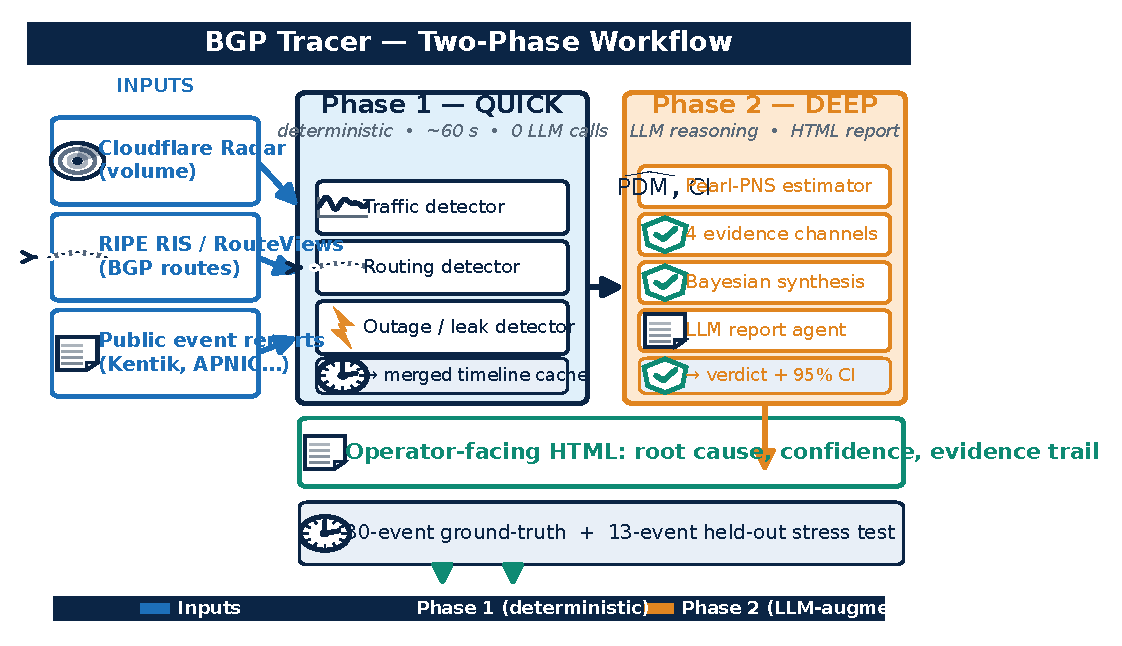
\includegraphics[width=\linewidth]{figs/fig1_workflow.pdf}
\caption{BGP Tracer end-to-end workflow. The shared
cache is the single point of interpretability: every
verdict is traceable to a detector output, and every
degraded-mode behaviour is recorded in the cache. The
coarse screen is the load-reduction mechanism; the
two-phase analysis (deterministic arbitration, then
Pearl-PNS causal attribution) is the core contribution.}
\label{fig:workflow}
\end{figure*}

The rest of this section walks through the system in the order an
operator encounters it. Section~\ref{sec:overview-architecture}
introduces the agents and the substrate they share.
Section~\ref{sec:overview-phase1} describes Phase 1, where the
routing and traffic signals are put on a common grid and reduced to
a five-class correlation verdict. Section~\ref{sec:overview-phase2}
describes Phase 2, where the causal engine attributes direction and
cause type. Section~\ref{sec:overview-degraded} closes with the
degraded modes that make the system safe to run unattended.

\subsection{Architecture and agents}
\label{sec:overview-architecture}

Four agents produce evidence, and one workflow engine decides what
runs next.

\textbf{Traffic agent.} The traffic agent owns the entire data-plane
side. It pulls five-minute aggregate traffic series for the AS under
analysis, establishes a periodic baseline against historical windows,
and runs a family of complementary detectors over the de-trended
series: a statistical $3\sigma$ test against the historical mean and
standard deviation, an isolation-forest density test, a sudden-drop
test, a sustained-outage test, a peak-to-trough excursion test, and a
percentile-envelope test. The detectors are combined under an OR rule
with a context filter that removes anomalies whose deviation from the
historical baseline is below 30\%, which is what keeps ordinary
day/night cycling from being reported as an incident. The agent's
output is a structured argument: a list of anomalous buckets, the
baseline method used, the periodicity confidence, and the magnitude of
the excursion.

\textbf{Routing agent.} The routing agent owns the control-plane side.
It runs three detectors whose structural signals are complementary.
\msbd{} (multi-scale breakpoint detection) locates the moment the
routing series changes regime, which is the intervention point that
Phase~2 anchors on. \ctpr{} (constrained path validation) scores
announcements against the Gao--Rexford valley-free constraint and the
AS-path length expectation, which is the structural signature of a
route leak. \cic{} (cascade impact computation) propagates the
detected anomaly along the CAIDA AS-relationship graph to determine
which ASes are downstream, weighting each hop by its commercial
relation so that a customer's traffic is not conflated with a peer's.

\textbf{Reasoning agent.} The reasoning agent runs the causal
attribution engine (Section~\ref{sec:overview-phase2}). It consumes
the routing and traffic arguments and produces a causal direction, a
cause type, a posterior over the three direction hypotheses, and an
explicit abstention record when the evidence does not support a
commitment.

\textbf{Report agent.} The report agent renders a human-facing
narrative. It consumes the cache and never writes verdicts: the LLM
layer is a narrative renderer, never a verdict source
(Section~\ref{sec:impl}).

\textbf{Shared cache.} The four agents communicate through a
versioned, content-addressed cache rather than through direct calls.
Every detector output, every gate transition, and every degraded-mode
behaviour is written as an immutable record. This arrangement is what
makes a verdict replayable: re-running the analysis on the same inputs
reproduces the same verdict bit for bit (Section~\ref{sec:impl}).

\subsection{Phase 1: Event--traffic correlation}
\label{sec:overview-phase1}

Phase 1 answers one question: \emph{does this routing event have
traffic impact?} It is a two-stage coarse-to-fine pipeline, and the
coarse stage exists to make the fine stage affordable.

\textbf{Stage 1 -- Coarse screen.} The traffic agent pulls five-minute
traffic aggregates from Cloudflare Radar~\cite{cloudflare-radar} and
compares the event window against the same window one and two weeks
earlier, which removes the weekly and daily periodic components without
an explicit seasonal decomposition. Two statistics drive the screen:
the relative shift in the mean traffic level and the ratio of
in-window dispersion to baseline dispersion, which together capture a
level change and a volatility spike respectively. Each statistic that
exceeds its published threshold contributes a fixed weight to a quick
score; the score itself is the screen's output. A candidate is admitted
to Stage 2 iff the score clears the admission threshold. The rejection
reason is recorded in the cache; a refusal-to-score is a verdict, not
silence.

\textbf{Stage 2 -- Fine-grained pass.} For each admitted candidate, the
traffic agent computes the periodic baseline and deviation series; the
routing agent runs the three control-plane detectors (\msbd{}, \ctpr{},
\cic{}) and writes structured outputs to the shared cache. The
arbitration reduces these to a \textbf{five-class verdict} through three
layered principles: suspension (a detector with no evidence is
suspended, not silenced), evidential gating (each candidate must clear a
minimum hit count and score), and temporal correlation (whether routing
and traffic anomalies overlap in time). Six disambiguation rules
resolve residual overlaps in a fixed design-time order
(Appendix~\ref{app:arbitration}).

\textbf{Phase 1 output.} Phase 1 returns a correlation verdict from five
classes:
\begin{itemize}
    \itemsep0pt
    \item \texttt{real\_incident}: both routing and traffic signals present and temporally correlated --- \textbf{trigger Phase 2}
    \item \texttt{silent\_alert}: routing signal present, traffic absent
    \item \texttt{traffic\_only}: traffic signal present, routing absent
    \item \texttt{correlation\_uncertain}: both signals present but temporally misaligned --- \textbf{trigger Phase 2}
    \item \texttt{no\_clear\_anomaly}: neither signal present --- pipeline short-circuits
\end{itemize}
Phase 1 does \emph{not} output the cause type (outage / route\_leak /
origin\_hijack). That is the role of Phase 2, which runs the causal
attribution engine on \texttt{real\_incident} and
\texttt{correlation\_uncertain} verdicts. The two phases are
independent: Phase 1 does not consult Phase 2, and Phase 2 consumes the
Phase 1 verdict without overwriting it.

\subsection{Phase 2: Causal attribution}
\label{sec:overview-phase2}

Phase 2 is invoked only for \texttt{real\_incident} and
\texttt{correlation\_uncertain} verdicts. It answers two questions:
(1) what is the causal direction between the routing anomaly and
traffic anomaly (R$\to$T or T$\to$R)? and (2) what is the cause type
(outage, route leak, or origin hijack)?

\textbf{One estimator, two directions.} \pdm{} and CSS are \emph{the
same functional form} evaluated under two different interventions, not
two competing estimators. The single estimator is
\begin{equation}
    \mathrm{CSS}(X \to Y) = \hat{E}[Y \mid do(X{=}1)] - \hat{E}[Y \mid do(X{=}0)], \label{eq:css-def}
\end{equation}
a pre/post difference-in-means in which the pre-window is the synthetic
control. \pdm{} is \eqref{eq:css-def} instantiated with $(X,Y)=(R,T)$ and
the intervention point set to the MSBD routing breakpoint; CSS is the
same quantity instantiated with $(X,Y)=(T,R)$ and the intervention point
set to the traffic breakpoint. Reporting them as two named estimators
would imply a methodological distinction that does not exist; what
differs is only \emph{which series defines the intervention window}.

\textbf{The commit gate.} The favoured direction is committed only when
the bootstrap 95\% CI of that direction excludes zero~\cite{efron-1979-bootstrap}
and the permutation $p$-value is below $0.05$~\cite{phipson-2010-permutation};
the engine otherwise abstains. When the two series are temporally
ordered, precedence alone disqualifies the reverse direction, since a
cause cannot follow its effect. Abstention is the default rather than
the exception.

\textbf{Why a pre/post estimator rather than full Pearl do-calculus.}
Pearl's do-calculus rules require a known causal graph and a suitable
adjustment set~\cite{pearl-causality-2009,spirtes-cps-2000}. BGP
telemetry carries no a priori causal graph: BGP updates and traffic are
jointly produced by operator decisions whose structural relationship is
exactly what the analyst lacks. The pre/post partition at the routing
breakpoint is the standard graph-free identification. We therefore
describe PDM as \emph{Pearl-PNS-anchored}: the framework supplies the
counterfactual interpretation, the identification is approximate without
a graph, and the abstention gate makes the approximation
auditable~\cite{pearl1999,shpitser-2008-pns}.

\textbf{Five evidence channels.} Phase 2 aggregates five evidence
channels in a composite Bayesian synthesis (Appendix~\ref{app:abstention}).
Each channel is a hypothesis test on the pre/post partition: (1) MSBD
tests whether the routing breakpoint coincides with a traffic drop;
(2) CTPR tests whether the AS-path anomaly scope covers the candidate
AS; (3) CIC tests whether the routing cascade reaches beyond the
candidate AS, propagating along the CAIDA AS-relationship graph and
weighting each hop by its commercial relation so that a customer's and
a peer's traffic are not conflated; (4) Granger tests linear predictive
causality~\cite{granger-1969-investigating}; (5) transfer entropy tests
information-theoretic causality~\cite{schreiber-2000-te,besserve-2010-te}.
The posterior is $P(d \mid E) \propto P(d) \prod_{ch} \mathrm{LR}_{ch}(d)$
over $d \in \{R \to T,\, T \to R,\, \text{independent}\}$, so a channel
that disagrees with the anchor is discounted rather than outvoted.

The abstention threshold $\tau=0.34$ is a natural boundary: three
equiprobable hypotheses give a uniform prior of $1/3$, so $\tau > 1/3$
means the dominant hypothesis outweighs the other two combined.
Abstention is therefore not an arbitrary design choice but a
consequence of the prior.

\textbf{Abstention is auditable.} The engine abstains at three levels:
the estimator level, where a CI crossing zero or a permutation
$p$-value above threshold blocks the commit; the channel level, where a
best-direction confidence below the floor leaves the direction unknown;
and the synthesis level, where a dominant posterior at or below $\tau$
yields an unknown verdict. Each is recorded in the cache with its
triggering statistic, so an abstention is a verdict with a stated reason
rather than silence.

\subsection{Degraded modes}
\label{sec:overview-degraded}

Each input source is a first-class degraded mode. Missing traffic data
reduces Phase~1 to a routing-only verdict; missing routing data reduces
it to the outage detector only; Phase~2 gracefully reduces to the
available channels. A partial verdict is more useful than no verdict,
but only when explicitly marked as partial in the cache. The
cache therefore records not only the verdict but the set of channels
that produced it, so an operator can always tell a confident verdict
from a confident verdict computed on half the evidence.
